\section{Introduction}

\begin{figure}[]
  \centering
  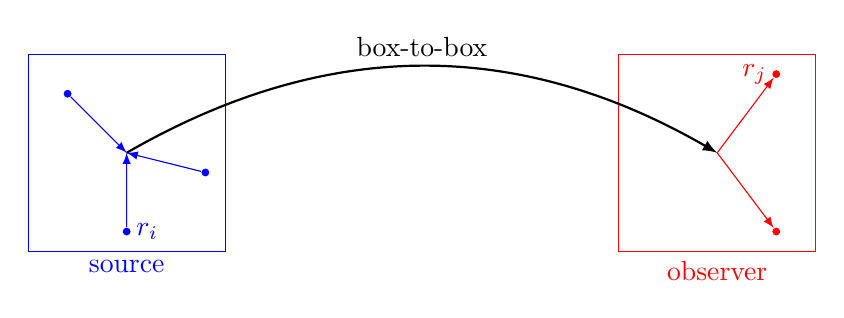
\begin{tikzpicture}[scale=2.5, >=latex]
  \draw[color=blue] (0, 0) rectangle (1, 1);
  \draw[color=red] (3, 0) rectangle (4, 1);

  \draw[color=blue] (0.2, 0.8) node[circle, fill, inner sep=1pt](s1){};
  \draw[color=blue] (0.5, 0.1) node[circle, fill, inner sep=1pt](s2){};
  \node[blue, anchor=west] at (s2) {$\vb{r}_i$};
  \draw[color=blue] (0.9, 0.4) node[circle, fill, inner sep=1pt](s3){};

  \draw[color=red] (3.8, 0.9) node[circle, fill, inner sep=1pt](o1){};
  \node[red, anchor=east] at (o1) {$\vb{r}_j$};
  \draw[color=red] (3.8, 0.1) node[circle, fill, inner sep=1pt](o2){};

  \draw[color=blue, ->] (s1) -- (0.5, 0.5);
  \draw[color=blue, ->] (s2) -- (0.5, 0.5);
  \draw[color=blue, ->] (s3) -- (0.5, 0.5);

  \draw[color=red, ->] (3.5, 0.5) -- (o1);
  \draw[color=red, ->] (3.5, 0.5) -- (o2);

  \draw[->, thick] (0.5, 0.5) to [bend left] node[pos=0.5, above]{box-to-box} (3.5, 0.5);

  \node[blue, anchor=north] at (0.5, 0) {source};
  \node[red, anchor=north] at (3.5, 0) {observer};
\end{tikzpicture}

  \caption{General principle of mathematically accelerated \textcolor{red}{techniques}.
    Given a sufficiently smooth Green's function, we can aggregate distant sources to significantly reduce the overall computational complexity.
  }
  \label{fig:box to box}
\end{figure}

We wish to accelerate the (discrete) calculation of 
\begin{equation}
  \vb{E}(\vb{r}, t) = \iint_{} g(\vb{r} - \vb{r}'; t - t') \vb{J}(\vb{r}', t') \dd[3]{\vb{r}'} \dd{t'}
  \label{eq:general integral equation}
\end{equation}
between a set of source and observation points (often---but not necessarily---coincident).
Here, $\vb{E}$, $g$, and $\vb{J}$ represent a field, propagator, and source distribution and each can have a number of different properties (such as bandlimitedness or a dyadic structure) depending on the physics under consideration.
Algorithms such as the fast-multipole (FMM)~\cite{Greengard1987} and plane-wave time-domain (PWTD)~\cite{Ergin1999} methods enjoy widespread success in accelerating \cref{eq:general integral equation} and operate by decomposing a composite Green's function into a product of factors and a translation function, e.g.\ $g(\vb{r} - \vb{r}') = \sum_i b_i(\vb{r}' - \vb{r}_o) T(\vb{r}_s - \vb{r}_o) a_i(\vb{r}_s - \vb{r})$.
Using this representation, the $a_i(\vb{r}_s - \vb{r})$ and $b_i(\vb{r}' - \vb{r}_o)$ functions become aggregation and disaggregation operations for sources in the vicinity of $\vb{r}_s$ and $\vb{r}_o$.
By transmitting these aggregated quantities between $\vb{r}_{s,o}$ points, \textcolor{red}{fill this in} \cref{fig:box to box}.
Unfortunately, as kernel-dependent methods, these techniques rely heavily on the mathematical details of $g(\vb{r} - \vb{r}'; t - t')$ as the solution to a partial differential equation (a proper Green's function) to determine a convergent decomposition.
The frequency-shifted propagators developed in \cref{ch:quantum dots} do not arise from rigorous mathematical analysis, instead coming from assumptions made about the underlying radiative system, thus we must seek algebraic acceleration techniques instead.

For discrete, causal systems, the translational invariance (in time) of \cref{eq:general integral equation} implies $\vb{E} = G \cdot \vb{J}$, or
\begin{equation}
  \mqty(\vb{E}_0 \\ \vb{E}_1 \\ \vb{E}_2 \\ \vb{E}_3 \\ \vdots \\ \vb{E}_{N_t - 1}) = 
  \mqty(G_0 \\ G_1 & G_0 \\ G_2 & G_1 & G_0 \\ G_3 & G_2 & G_1 & G_0 \\ \vdots & \ddots & \ddots  & \ddots & \ddots \\ G_{N_t - 1} & \dots & G_3 & G_2 & G_1 & G_0) \cdot
  \mqty(\vb{J}_0 \\ \vb{J}_1 \\ \vb{J}_2 \\ \vb{J}_3 \\ \vdots \\ \vb{J}_{N_t - 1})
  \label{eq:matrix system}
\end{equation}
Here, the numerical index represents the evolution of time and thus the $G_i$ denote block matrices that govern the spatial interactions of the basis functions.
(For electromagnetic systems of finite size, the $G_{i' > i} = 0$ for some $i$ due to the retarded nature of $g(\vb{r} - \vb{r}'; t - t')$.)

The accelerated method---derived from ``Adaptive Integral Method'' (AIM) techniques in both frequency~\cite{Bleszynski1996} and time-domain~\cite{Yilmaz2004} applications---proceeds by decomposing $G$ into terms describing near and far-field effects (i.e. $G = G_\text{near} + G_\text{far}$).
As each source has a limited number of near-field neighbors independent of the size of the system, $G_\text{near} \cdot \vb{J}$ proceeds exactly as in \cref{ch:quantum dots} and needs no (mathematical) acceleration.
Evaluation of the far-field, however, uses a compressed representation of $G_\text{far}$ alongside a fast matrix-vector multiplication to achieve an $\mathcal{O}(n \log n)$ spatial complexity (as compared with the na\"ive $\mathcal{O}(n^2)$ strategy).

\begin{figure}
  \centering
  \conditionalFigureInput{figures/toeplitz_matrix}
  \caption{\label{fig:toeplitz}Illustration of the three-level (corresponding to three spatial dimensions) Toeplitz matrix structure for a $1/r$ propagation kernel on a $5 \times 5 \times 5$ grid.
  As all of the unique elements lie along the first column, an FFT diagonalizes the ``circulant equivalent'' matrix (formed by mirroring appropriate elements/blocks) in $\mathcal{O}(n \log n)$ time.}
\end{figure}
